\section{Architecture}

A program can be represented in several ways. There is extensive reading material on how logical programming can be used to represent and analyse programs\cite{Reps1995}\cite{DatalogDBQueries}. However, other approaches exist that lean more closely towards the implementation of our system.  As discussed in section \ref{subsec:staticAnalysis}, static analysis can be a means of representing implicit and explicit information about a piece of source code. For our approach, we needed a representation containing enough information to look up non-trivial properties about how information and data flows in the program. Abstract interpretation of a program produces an abstract state graph that meets these requirements. The graph contains information about control- and data flow, providing a rich source of information that can be extracted through some query language and a querying mechanism. 

% Querying mechanisms -> approaches in datalog queries enzo
Querying programs depends greatly on the way a program is represented and how queries are transformed into query-engine-friendly data structures. One way would be to resolve queries using existing techniques such as \cite{bddbddb}. This technique matches queries expressed in Datalog against a database of rules representing the relations of an entire program. Since our approach represents programs as flow graphs, an alternative method to resolve queries needs to be applied. A suitable algorithm to solving queries is presented in \cite{algoEngine}, which enables us to query flow graphs directly. The internals of this algorithm will be discussed in greater detail in section \ref{subsec:matchingEngine}.

% DSL
It is important that exploring and accessing information of a flow graph happens in an easy and user-friendly way. We believe regular path expressions to be the most legible way to write clean and understandable queries. With the JS-QL language, we offer an internal domain-specific language specialized in expressing queries corresponding to sequences of states in the flow graph. 

The actual architecture of the JS-QL framework is depicted in figure \ref{fig:architecture}. The query engine takes as input (i) a flow graph and (ii) a query, written in the JS-QL language. The output will consist of tuples \texttt{<State, Substitutions>} for all paths on which a match for the query was found.

\begin{figure}
    \centering
      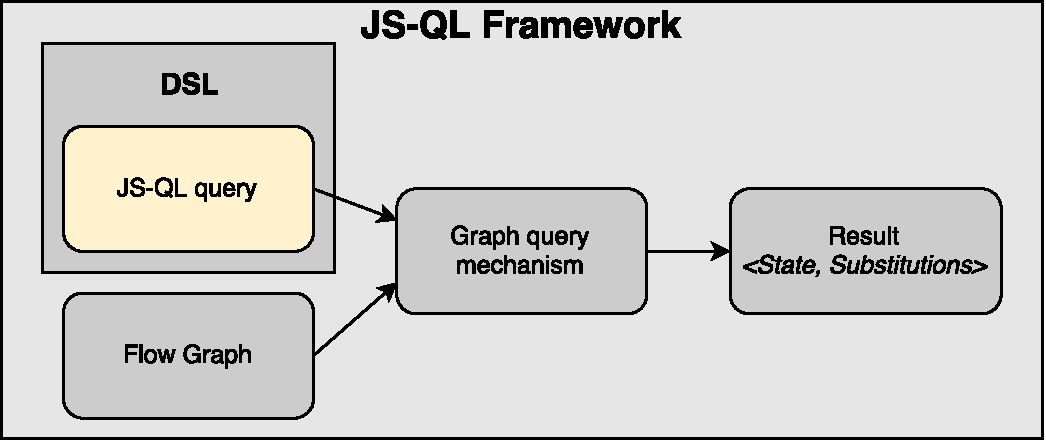
\includegraphics[width=0.9\textwidth]{images/Architecture} 
      \caption{JS-QL framework architecture}
    \label{fig:architecture}
\end{figure}
\section{Flow graphs for JavaScript programs}

The need for detailed control- and data flow information in our program representation graph limits the types of graphs that can be used for our framework. Program dependence graphs\cite{PDG} for example can be very useful to track the flow of information between certain points in a program but often lack more general information about program states, making them less qualified to use as our main program representation. In contrast, the JIPDA\cite{} abstract state graph contains all the information needed to precisely express patterns to be detected in a program. This section takes an in-depth look at the JIPDA abstract state graph and the information it holds in its states. Figure \ref{fig:JipdaGraph} shows part of a typical graph produced by JIPDA for a program containing a check for whether a number is equal to zero or not.

As can be observed, the graph depicts all possible paths a program can traverse. Since the analysis in JIPDA is flow-sensitive, it is guaranteed that a state \texttt{a} on some path in the graph occurs before a state \texttt{b} on the same path if state \texttt{a} occurs first before state \texttt{b} on the path. This makes reasoning about patterns in a program much easier, since no false positives will occur with regards to the order of execution of states. The graph produced by the JIPDA analysis is also a flow graph, and more precisely maintains information about two types of flows:
%TODO uitleggen flow graph value flow en control flow -> in JIPDA

\begin{enumerate}
\item \textit{data flow}: Information about what values an expression may evaluate to.
\item \textit{Control flow}: Information about which functions can be applied at a call site.
\end{enumerate}

We need these kinds of information to be able to make correct assumptions at certain states in a program. Consider the expression \texttt{f(x)} for example. Function \texttt{f} will be the function that is invoked. The value of \texttt{f} however may depend on other operations that occur before this function call, such as another function call. Therefore it is important to know which function(s) \texttt{f} may refer to, illustrating the need of control and data flow.

\subsection*{States of an abstract state graph}

The abstract state graph is an alternation of four different types of states. JIPDA internally uses Esprima\cite{Esprima} to parse JavaScript code and set up an abstract syntax tree (AST). This AST is the starting point for the analysis that JIPDA performs, hence information about the nodes from the AST is also contained in certain states in the resulting graph. These states are marked in red and are so-called \textit{evaluation states}. Other states are \textit{continuation states} (green), \textit{return states} (blue) and \textit{result states} (yellow).

\begin{figure}[!ht]
    \centering
      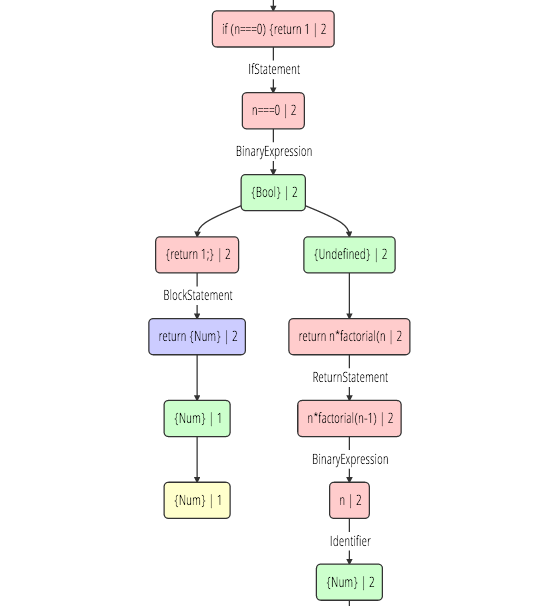
\includegraphics[width=262px, height=606px, keepaspectratio]{images/JipdaGraph} 
      \caption{Example JIPDA abstract state graph}
    \label{fig:JipdaGraph}
\end{figure}

%HELP VRAGEN BIJ JENS
\begin{enumerate}
\item \textit{Evaluation state}: Represents the evaluation of an expression or statement in the program.
\item \textit{Continuation state}: ...
\item \textit{Return state}: Indicates the return of a function application, having the returned value stored in one of its properties.
\item \textit{Result state}: Final state of the graph, indicating the abstract final value(s) of the program. The graph can have more than one result state, depending on the program's nature. 
\end{enumerate}

These states all contain valuable information about the point in the program they represent. The next part of this section discusses the different attributes that can be found in the states of the abstract state graph. 

%Kont, Lkont, Node, Benv, Store, Value
\subsection*{Node}

As said earlier, evaluation states contain information about the expression or statement they represent in the program. This information is stored in the form of an AST node, as obtained by the Esprima parser. Detailed information about the current expression or statement can be found in the properties of these nodes. Our approach makes extensive use of this information to find a match for a specified pattern along the graph. Note that node information is exclusively available in evaluation states. If we parse the following program \\\\
\texttt{function answerToTheUniverse(arg)\{}\\
\phantom{ }\phantom{ }\phantom{ }\phantom{ }\texttt{return 42;}\\
\texttt{\}}\\
\\
we obtain its corresponding JSON representation, listed in \ref{lst:EsprimaTree}.
\\
\begin{lstlisting}[label={lst:EsprimaTree},language=JSON,caption=Parsed JavaScript program AST, mathescape=true]  % float=t?

{
    "type": "Program",
    "body": [
        {
            "type": "FunctionDeclaration",
            "id": {
                "type": "Identifier",
                "name": "answerToTheUniverse"
            },
            "params": [
                {
                    "type": "Identifier",
                    "name": "arg"
                }
            ],
            "defaults": [],
            "body": {
                "type": "BlockStatement",
                "body": [
                    {
                        "type": "ReturnStatement",
                        "argument": {
                            "type": "Literal",
                            "value": 42,
                            "raw": "42"
                        }
                    }
                ]
            },
            "generator": false,
            "expression": false
        }
    ]
}
\end{lstlisting}

The parsed source code is a list of nodes contained in the body property of the "program" AST node. This is in fact the root node of the AST. Each node has its own \textit{type} that distinguishes different kinds of expressions and statements. The example code in \ref{lst:EsprimaTree} shows that the parsed code is a "FunctionDeclaration" with its own id, parameters, defaults and body attributes. We observe that the attributes in turn can again be (a list of) nodes.

\subsection*{Binding environment and store}

In JIPDA, variables point to addresses. The mapping of a variable to an address is called a \textit{binding}. These bindings reside in a \textit{binding environment $\hat{\beta}$}. Each binding maps to a value through the \textit{store} $\hat{\sigma}$. The store acts as a heap where bindings represent addresses on that heap. Being able to capture bindings, addresses and values in metavariables enables us to express and inspect data flow properties of programs. Variables are mapped to values in two stages. The first step for looking up a variable $\hat{\nu}$ is to locate its binding in $\hat{\beta}$. Next, the value of the variable can be looked up in the store by composing these two functions. The value of $\hat{\nu}$ is given by $\hat{\sigma}(\hat{\beta}(\hat{\nu}))$. This way of mapping variables to values allows us to reason about individual bindings, which is necessary because during interpretation multiple bindings to the same variable can exist simultaneously. Listing \ref{lst:benvStoreExample} gives an example of how a variable gets a binding and is later looked up.
\\
\begin{lstlisting}[label={lst:benvStoreExample},language=JavaScript,caption=Example of the binding environment and store workings, mathescape=true]  % float=t?

function f(){
  //$\hat{\beta}$ contains a binding $x \rightarrow \widehat{Addr}$
  var x = 3; 
  
  //$\hat{\sigma}$ has an entry $\widehat{Addr} \rightarrow \widehat{Val}$
  //and the (set of) corresponding value(s) for x is returned. 
  return x;
}
var value = f();
\end{lstlisting}


\subsection*{Value}
%Value uit store
The lookup of a variable through a binding in the store results in the (set of) value(s) for that variable. This information is available in all states but evaluation states. For continuation states, the value will represent the looked up or calculated values of an expression. A return state's value is the set of possible values that will be returned. Result states contain the final values of a program.

\subsection*{Application context}

Some text about the application context.

\subsection*{Stack}

Some text about the stack.





\section{External DSLs for querying graphs}
%Intro http://www.st.ewi.tudelft.nl/~arie/papers/dslbib.pdf

For almost any branch of science and engineering we can distinguish between two types of approaches. One type of approach is the \textit{generic} approach, which offers solutions to a wide range of problems within a certain domain. However, these solutions are often suboptimal. When we reduce the set of problems we want to solve, an often better approach to solving these problems would be the \textit{specific} approach.
In software engineering terms these two approaches translate to two types of languages: General purpose languages (GPLs) and domain-specific languages (DSLs) respectively. 
\textit{Domain-specific language} is no new concept. Many programming languages that are now considered general purpose language started out as domain-specific languages. Cobol, Fortran and Lisp for example all came into existence as dedicated languages for solving problems in a certain area\cite{vanDeursen:2000}, but gradually evolved into the full fledged languages they are today. The rest of this section is devoted to the comparison of GPLs and DSLs, in which we advocate that DSLs are the best approach for the instantiation of the JS-QL framework. We further give an overview of related work about DSLs for querying graphs and DSLs in general.


\subsection{Domain-specific language vs. general purpose language}
%Wat is een DSL & wat is een GPL
%Over GPL wat FLuent-interfaces zegt! 'divide en conquer limited ...;'

Before we start this comparison, we give a formal definition of domain-specific languages and general purpose languages:
\begin{definition}
    A \textit{domain-specific language} (DSL) is a programming language of executable specification language that offers, through approproate notations and abstractions, expressive power focused on, and usually restricted to, a particular problem domain.
\end{definition}

\begin{definition}
    A \textit{general purpose language} (GPL) is a programming language that is broadly applicable across application domains, and lacks specialized features for a particular domain.
\end{definition}

The key focus for DSLs are its focussed expressive power. The expressiveness of DSLs comes from the fact that they were created to solve a small set of problems. They offer a high-level set of mechanisms for the programmer to express his ideas for a particular application domain. A DSLs aim is to have the language focus specifically on those aspects and concepts that are relevant to a particular problem domain, hiding all boilerplate code that comes along with GPLs. Designers of general purpose programming languages also try to help the programmers express their ideas concisely and clear, but even with the most elegant programming language difficulties arise when programs get bigger and more complex. To this extent, extra features were developed for GPLs to further abstract code and reduce complexity. Amongst these features are functions, subroutines, packages, objects \dots  Even though these features are useful for general applications, the languages that implement them often have a set of operational baggage associated with them which makes a program unneccesarily complex to develop\cite{FluentInterfacesJava}. 

In contrast to the generic approach, the domain-specific approach to language design makes it possible to allow low-level system requirements to guide the design of the required high-level language features one wishes to incorporate into his language, instead of being required to use existing general-purpose designs.
We therefore believe that a domain-specific language is the best pick for our query language.
Benefits of domain-specific languages include:

\begin{itemize}
\item DSLs are application-specific. This allows users to express their ideas at the level of abstraction of the problem domain.
\item DSL programs are concise, self-documenting and highly reusable\cite{Bentley:1986}
\item DSLs enhance productivity, maintainability, portability and reliability
\item DSLs can shift the development of systems from typical system developers to domain experts with deeper knowledge of the domain.
\item DSLs contain domain knowledge which can be reused
\item DSLs significantly reduce programming errors
\end{itemize}

\noindent Some counterarguments for using a DSL are:
\begin{itemize}
\item The cost of designing, implementing and maintaining a DSL
\item The cost of educating DSL users
\item A DSL has limited applicability
\item The difficulty of finding the correct scope for a DSL
\end{itemize}

We argue that the costs for setting up a DSL do not weigh up against the benefits of a DSL. The high reusability alone makes up for the one-time investment of designing and implementing the language. When developing a language for a certain domain, naturally its applicability will be limited to that domain only, as this is the purpose of a domain-specific language. Finding the correct scope for a DSL might be cumbersome, but there is a great amount of literature about specifying the domain of a problem\cite{Simos:1995} and the domain for DSLs\cite{karsai2014design}\cite{gunther2010agile}. 

\subsection{External DSLs}

Many DSLs come along with a compiler which translates DSL programs into applications. These kinds of DSLs are called \textit{external} DSLs. the compiler is also called an application generator\cite{Cleaveland:1988}, whereas the DSL is the application-specific language. The main advantage external DSLs is that the implementation of the compiler can completely be tailored to the DSL. The DSL in turn is restricted in no way with regards to notation, primitives and the like because its syntax is independent of the underlying language (since there is none). The remainder of this section discusses existing work about external DSLs used for graph traversal and graph querying.

\subsection*{StruQL}

StruQL is the query language behind the Strudel system\cite{Fernandez97aquery}. The language is built to support the retrieval and construction of data for web sites. This data is represented as \textit{data graphs} and originates from external sources, the integrated view and the web site itself. These data graphs depict web sites as nodes, representing web pages or atomic values, interconnected with directed, labelled edges. These edges then represent the links or attribute values that connect two nodes. The language enables users to create and query data graphs, but the real power of StruQL lies in their ability to express regular path expressions. This allows for very flexible queries describing the paths about which information needs to be accessed in great detail.
It also allows to compute the transitive closure of an \textit{arbitrary 2n-ary} relation, meaning that it can compute all reachable nodes from a certain node for any input graph. Buneman et al\cite{Buneman:1996} have formally proven that this is not a trivial computation.

\subsection*{GraphQL}
%http://sites.fas.harvard.edu/~cs265/papers/he-2008.pdf -> GraphQL

GraphQL\cite{He:2008} is a query language which allows to query graph databases. The language uses a graph pattern as a basic operational unit. These graph patterns consist of a graph structure and a predicate on attributes of the graph. They introduced the notion of formal languages for graphs. This is useful for composing and manipulating graph structures and is used as a basis of the graph query language.
The core of the language is a graph algebra in which the selection operator is generalized to graph pattern matching and a composition operator is introduced for rewriting matched graphs. In terms of expressive power, the language is contained in Datalog. This means that every query in GraphQL can be converted to a Datalog query. The language allows users to express concatenation, disjunction and recursion, allowing users to write dynamic queries. They address the NP-completeness of subgraph isomorphism by using neighborhood subgraphs and profiles, joint reduction of the search space, and optimization of the search order.

\subsection*{ASTLOG}
%http://www.cs.nyu.edu/~lharris/papers/crew.pdf

\subsection*{Lorel}
%http://infolab.stanford.edu/lore/pubs/lorel96.pdf -> Semistructured data

%-----------------------------
%RW over EDSL los van graphs:
%http://graphics.stanford.edu/hackliszt/liszt_sc2011.pdf
%http://homepages.cwi.nl/~jurgenv/papers/SCAM-2009.pdf
%https://www.researchgate.net/publication/220071161_BDL_A_Specialized_Language_for_Per-Object_Reactive_Control
%Chandra1999
%-----------------------------


\subsection{Internal DSLs}
%It was coined by Hudak\cite{Hudak:1996}
%eerste keer door Hudak -> http://citeseerx.ist.psu.edu/viewdoc/download?doi=10.1.1.49.6020&rep=rep1&type=pdf
% Embedded kan GPL gebruiken. -> Sometimes, however, they contain an entire general-purpose language (GPL) as a sublanguage, thus offering domain-specific expressive power in addition to the expressive power of the GPL. This situation occurs when DSLs are implemented as embedded languages
%Waarom internal
%----------------
%RW over DSEL graph traversal:
\subsection*{Gremlin}
%http://arxiv.org/pdf/1508.03843.pdf -> Graph traversal
\subsection*{Dagoba}
%Dagoba
\subsection*{A little language for surveys}
%Survey language -> illustrates flexibility of embedded dsl + design patterns
%
%-----------------------------
%RW over DSEL los van graphs:
%https://www.usenix.org/events/dsl99/full_papers/jennings/jennings.ps
%https://www.usenix.org/legacy/publications/library/proceedings/dsl97/full_papers/stevenson/stevenson.pdf
%http://haskell.cs.yale.edu/wp-content/uploads/2011/02/padl99.pdf
%Eliott1999
%https://www.usenix.org/legacy/publications/library/proceedings/dsl97/full_papers/kamin/kamin.pdf
%-----------------------------

%2 die ik al had -> 1 ervan queriet graphs!

%https://idl.cs.washington.edu/files/2014-Ellipsis-EuroVis.pdf --> Zij doen wel element van fluent API als argument -> Overwegen of gebruiken of niet
% MISSCHIEN http://www.cs.um.edu.mt/gordon.pace/Research/Papers/wict2009-01.pdf

%HIER NOG ZETTEN WAAROM INTERNAL GEKOZEN (overhead van compiler enz..., out of scope van dissertation)


\section{Design of an internal DSL for querying flow graphs}

%zie Domain-specific languages: An annotated Bibliography
%-> DSL sometimes contains entire GPL as sublanguage ...

\subsection{internal DSL design constraints}

%CONSTRAINTS:
% What is the problem domain? -> Domein afbakenen kan via http://citeseerx.ist.psu.edu/viewdoc/download?doi=10.1.1.49.9877&rep=rep1&type=pdf
%-> daarom ook voor DSL gekozen
%Flow graphs beperken predikaten, Extensibility, JavaScript, no REPL
%https://idl.cs.washington.edu/files/2014-Ellipsis-EuroVis.pdf --> Zij doen wel element van fluent API als argument -> Overwegen of gebruiken of niet
\subsection{DSL implementation techniques}
%Welke bestaan er, welke hebben wij genomen
%3 delen beschreven in agile engineering

\subsection{DSL design patterns}
%Papers! http://martinfowler.com/dslCatalog/ (deferred evaluation enzo)

